\chapter{Proposta}
\label{cap:project}

\begin{quotation}[]{Yoko Ono}
The computer is my favourite invention. I feel lucky to be part of the global village. I don't mean to brag, but I'm so fast with technology. People think it all seems too much, but we'll get used to it. I'm sure it all seemed too much when we were learning to walk.
\end{quotation}

Com o objetivo de facilitar o acesso de usuários à fóruns, este trabalho traz como proposta um buscador que além de tratar a similaridade semântica, também leva em consideração a opinião da comunidade.
\section{Arquitetura}
% Todo usar figuras genéricas
%TODO Migração puxar de base de dados e envia para engenho de busca.
\begin{figure}[htb]
	\centering
	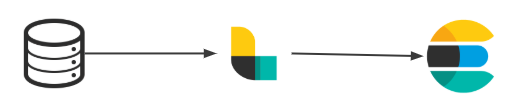
\includegraphics[width=\textwidth]{chapters/project/architecture.png}
	\caption{Arquitetura do sistema proposto}
\end{figure}
Neste projeto, será considerada uma arquitetura plugável à uma base pré-existente, a fim de manter a implantação do sistema o mais simples possível para que outros também possam o implementar em seus fóruns pré-existentes. 
A partir da base já existente do fórum, deve-se ter um serviço que trabalhe de forma contínua extraindo os dados e populando o engenho de buscas. O pré-processamento pode ser realizado tanto no serviço de migração ou no próprio engenho de busca. Entretanto, é essencial que o engenho de busca seja capaz de indexar e recuperar os dados armazenado de forma eficiente, conforme descrito nesse capítulo.

\section{Modelo Entidade Relacionamento}
\label{mer}

\begin{figure}[htb]
	\centering
	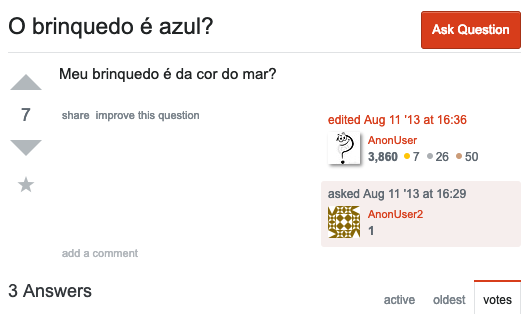
\includegraphics[width=\textwidth]{chapters/project/question-brinquedo.png}
	\caption{Exemplo de tópico}
	\label{fig:screenshootquestion}
	% TODO Verificar referências ao AskUbuntu
\end{figure}
Nos fóruns observados, foi percebido que os tópicos podem ter tanto título e corpo. Entende-se como corpo, o conteúdo textual descritivo da primeira postagem. Ao permitir que usuários votem indicado a utilidade ou qualidade de um documento, é adicionado um conceito de pontuação. Fóruns que não implementam recursos de avaliação, podem usar outros parâmetros para definir a pontuação de um documento, como número de visualizações ou alguma outra métrica de engajamento, por exemplo.

\begin{figure}[htb]
	\centering
	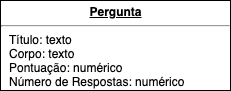
\includegraphics[scale=1.0]{chapters/project/mer.png}
	\caption{Formato exigido}
\end{figure}

\section{Pré-processamento}
Cada tópico passará por transformações antes de serem armazenadas. Considere os títulos descritas na tabela \ref{tab:example} no seu estado inicial. Estes irão ilustrar o pré-processamento. Vale ressaltar que o mesmo processo que está sendo descrito com os títulos também ocorre com o corpo.

\begin{table}[htb]
	\centering
    \def\arraystretch{1.2} % padding da linhas da tabela
    \begin{tabular}{|l|l|}
        \hline
        1 & <p>I will organize this room</p>            \\ \hline
        2 & All rooms are organized and clean \\ \hline
        3 & Cleaners are <b>very</b> effective                              \\ \hline
        4 & I will open this window                            \\ \hline
    \end{tabular}
	\caption{Frases de exemplo}
    \label{tab:example}
\end{table}


\subsection{Filtros de caracteres}
Na web é comum encontrar documentos com tags HTML. Para este projeto, estas tags não terão importância, portanto serão removidas e apenas será deixado apenas o texto. É possível verificar o resultado exemplificado na tabela \ref{tab:charfilter}.

\begin{table}[htb]
	\centering
    \def\arraystretch{1.2} % padding da linhas da tabela
    \begin{tabular}{|l|l|l|}
        \hline
        & \textbf{Antes} & \textbf{Depois} \\ \hline
        1 & <p>I will organize this room</p> & I will organize this room            \\ \hline
        2 & All rooms are organized and clean & All rooms are organized and clean \\ \hline
        3 & Cleaners are <b>very</b> effective & Cleaners are very effective                              \\ \hline
        4 & I will open this window & I will open this window                             \\ \hline
    \end{tabular}
	\caption{Frases de exemplo após os filtros de caracteres}
    \label{tab:charfilter}
\end{table}

\subsection{Tokenização}
O processo de tokenização é responsável por dividir um texto em unidades menores. Essas unidades podem ser palavras, caracteres, cadeia de palavras ou cadeia de caracteres. 

Para este projeto, foi usado a tokenização dividindo o conteúdo do texto em palavras usando o algoritmo Unicode Text Segmentation \cite{unicodesegmentation}.

\begin{table}[htb]
	\centering
    \def\arraystretch{1.2} % padding da linhas da tabela
    \begin{tabular}{|l|l|l|}
        \hline
        & \textbf{Antes} & \textbf{Depois} \\ \hline
        1 & I will organize this room & [I, will, organize, this, room]            \\ \hline
        2 & All rooms are organized and clean & [All, rooms, are, organized, and, clean] \\ \hline
        3 & Cleaners are very effective & [Cleaners, are, very, effective]                              \\ \hline
        4 & I will open this window & [I, will, open, this, window]                             \\ \hline
    \end{tabular}
	\caption{Frases de exemplo após a tokenização}
    \label{tab:tokenization}
\end{table}

\subsection{Filtros de tokens}
\subsubsection{Uniformização}
 Foi usada nesse projeto uma transformação responsável por deixar todos os caracteres minúsculos.

\begin{table}[htb]
	\centering
    \def\arraystretch{1.2} % padding da linhas da tabela
    \begin{tabular}{|l|l|l|}
        \hline
        & \textbf{Antes} & \textbf{Depois} \\ \hline
        1 & [I, will, organize, this, room] & [i, will, organize, this, room]            \\ \hline
        2 & [All, rooms, are, organized, and, clean] & [all, rooms, are, organized, and, clean] \\ \hline
        3 & [Cleaners, are, very, effective] & [cleaners, are, very, effective]                              \\ \hline
        4 & [I, will, open, this, window] & [i, will, open, this, window]                             \\ \hline
    \end{tabular}
	\caption{Frases de exemplo após as transformações}
    \label{tab:transformations}
\end{table}

\subsubsection{Remoção de Stop Words}
Existem palavras que adicionam pouco valor semântico ao texto, são conhecidas como \textit{stop words}. Stop words são palavras como: isso, um, a, o, que. Estas também serão removidas. Existem diversas formas de as detectar em um corpus, as mais comuns são com uso de listas com stop words predefinidas ou definindo um limiar máximo de ocorrências que uma palavra pode ter. Assume-se que palavras que ocorrem frequentemente em vários documentos não agregam muito conteúdo ao texto.

\begin{table}[htb]
	\centering
    \def\arraystretch{1.2} % padding da linhas da tabela
    \begin{tabular}{|l|l|l|}
        \hline
        & \textbf{Antes} & \textbf{Depois} \\ \hline
        1 & [i, will, organize, this, room] & [organize, room]            \\ \hline
        2 & [all, rooms, are, organized, and, clean] & [rooms, organized, clean] \\ \hline
        3 & [cleaners, are, very, effective] & [cleaners, effective]                              \\ \hline
        4 & [i, will, open, this, window] & [open, window]                             \\ \hline
    \end{tabular}
	\caption{Frases de exemplo após a remoção de stop words}
    \label{tab:tokenfilter}
\end{table}

\subsubsection{Stemming}
O propósito do stemming é reduzir a variação morfológica das palavras \cite{stemmingdef}. Documentos podem usar formas diferentes de uma palavra, por exemplo, um deles pode usar organizar, outro pode usar organizando e outro organizado. Embora as palavras não sejam idênticas, elas trazem consigo um sentido similar, o que pode ser útil em um sistema de recuperação da informação onde se deseja conteúdo relacionado, ainda que não idêntico.

\begin{figure}[htb]
	\centering
	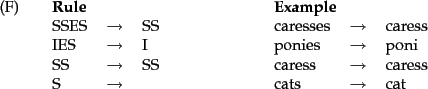
\includegraphics[width=\textwidth]{chapters/project/porterrules.png}
	\caption{Regras usadas na primeira fase do Porter Stemmer}
    \label{fig:porterstemmerprocess}
\end{figure}

O algoritmo mais comum de Stemming é o Porter \cite{porterstemming}. Este algoritmo usa fases com conjuntos definidos de regras para definir as transformações que uma dada palavra irá passar. A figura \ref{fig:porterstemmerprocess} mostra algumas das regras executadas na primeira fase do algoritmo.

Pode-se ver que agora, que as frases descritas na tabela \ref{tab:tokenfilter}, possuem mais palavras em comum do que anteriormente, isso garante uma busca mais abrangente, permitindo o usuário ter resultados com palavras diferentes da sua, mas que ainda acessem o mesmo domínio. Entretanto o resultado não é perfeito, palavras relacionadas podem acabar tendo finais diferentes e palavras diferentes podem possuir o mesmo resultado.
\begin{table}[htb]
	\centering
    \def\arraystretch{1.2}
    \begin{tabular}{|l|l|l|}
        \hline
        & \textbf{Antes} & \textbf{Depois} \\ \hline
        1 & [organize, room]  & [organ, room]            \\ \hline
        2 & [rooms, organized, clean]  & [room, organ, clean] \\ \hline
        3 & [cleaners, effective]  & [cleaner, effect]                              \\ \hline
        4 & [open, window]  & [open, window]                             \\ \hline
    \end{tabular}
	\caption{Frases de exemplo após o stemming}
    \label{tab:tokenfilter}
\end{table}

\subsection{Sumário}
Percebe-se na tabela \ref{tab:allphrases} o quanto cada uma das frases mudou e agora é possível verificar alguns padrões se repetindo onde não seria tão fácil se identificar previamente.
\begin{table}[htb]
	\centering
    \def\arraystretch{1.2} % padding da linhas da tabela
    \begin{tabular}{|l|l|l|}
        \hline
        & \textbf{Incial} & \textbf{Final} \\ \hline
        1 & <p>I will organize this room</p>  & [organ, room]            \\ \hline
        2 & All rooms are organized and clean  & [room, organ, clean] \\ \hline
        3 & Cleaners are <b>very</b> effective  & [cleaner, effect]                              \\ \hline
        4 & I will open this window  & [open, window]                             \\ \hline
    \end{tabular}
	\caption{Frases de exemplo ao final do pré-processamento}
    \label{tab:allphrases}
\end{table}

 Na tabela \ref{tab:quenstionpreprocessed} percebe-se o mesmo processo aplicado aos campos título e corpo de um tópico.

\begin{table}[htb]
	\centering
    \def\arraystretch{1.2} % padding da linhas da tabela
    \begin{tabular}{|l|l|l|}
        \hline
        & \textbf{Inicial} & \textbf{Final} \\ \hline
        \textbf{Título}              & O brinquedo é azul?            & [brinq, azul] \\ \hline
        \textbf{Descrição}               & Meu brinquedo é da cor do mar? & [brinq, cor, mar] \\ \hline
        \textbf{Pontuação}           & 7                              & 7 \\ \hline
    \end{tabular}
	\caption{Tópico após o pré-processamento}
    \label{tab:quenstionpreprocessed}
\end{table}     
\section{Indexação e Recuperação}
Concluído o pré-processamento, deve-se armazenar estes documentos, de forma que seja possível os recuperar em outro momento. Entretanto, métodos comuns encontrados na maioria dos bancos de dados são inadequados para lidar com texto.

Índices invertidos foram criados para serem uma forma rápida para lidar com dados massivos de texto. Para cada termo, é salvo o número de ocorrências e em que documentos eles ocorrem, conforme descrito na tabela \ref{tab:invertedindex}. Para cada campo de um tópico, existe um índice, ou seja, além do índice dos títulos na tabela \ref{tab:invertedindex}, ao realizar o pré-processamento do corpo, também haverá um índice para os corpos. 

\begin{table}[htb]
	\centering
    \def\arraystretch{1.2} 
    \begin{tabular}{|l|l|l|}
        \hline
        \textbf{Termo} & \textbf{Frequência} & \textbf{Documentos} \\ \hline
        organ & 2  & 1, 2            \\ \hline
        room & 1  & 2 \\ \hline
        clean & 1  & 2                              \\ \hline
        cleaner & 1  & 3                             \\ \hline
        effect & 1  & 3                             \\ \hline
        open & 1  & 4                             \\ \hline
        window & 1  & 4                             \\ \hline
    \end{tabular}
	\caption{Frases de exemplo no índice invertido}
    \label{tab:invertedindex}
\end{table}
Ao executar uma busca, o texto informado pelo usuário passa pelo mesmo processo de preprocessamento. Dessa forma, os tokens gerados ao final do pré-processamento serão usados para encontrar resultados na base que possuam um ou mais tokens em comum. Estes índices serão usados para também otimizar o processo de ranking, que o usará para avaliar a relevância de cada um dos termos.

\section{Ranking}
Na seção anterior, foi explicado como encontrar documentos relacionados. Nesta seção será explicado como definir a prioridade entre os selecionados, ou seja, determinar quais devem aparecer primeiro.

Será usado o algoritmo Okapi BM25, descrito no capítulo \ref{cap:informationretrieval}. Com o uso somente do cálculo de similaridade, já é possível ordenar os resultados. Entretanto, o Okapi BM25 não leva em consideração a pontuação adquirida pelo tópico, o que causa grandes impactos no resultado como será visto no capítulo \ref{cap:evaluation}. Devido à isso, é definida a relevância \textit{Rel} de um tópico \textit{x} para uma busca \textit{b} é definido pela média dos valores de similaridades obtidos pela função \textit{sim} da busca com título \textit{t} e da busca com corpo \textit{c} multiplicados com a pontuação \textit{p} obtida pelo tópico. Além disso, também é definido um parâmetro \textit{i} para regular a influência da similaridade no cálculo. Este cálculo é formalmente apresentado na equação \ref{eq:rel} e na tabela \ref{tab:relevance} é exemplificado o processo de ranking com dados fictícios.

\begin{equation}
    Rel(q, x) = \left(\frac{sim(t_{x}, b)  sim(c_{x}, b)}{2}\right)^{i}  p_{x} 
    \label{eq:rel}
\end{equation}

\begin{table}[htb]
	\centering
    \def\arraystretch{1.2} % padding da linhas da tabela
    \begin{tabular}{|l|l|l|l|l|}
        \hline
        Tópico & Sim. Título & Sim. Corpo & Pontuação & \textbf{Relevância} \\ \hline
        1 & 3 & 11 & 7 & 102487 \\ \hline
        2 & 0 & 1 & 1600 & 100 \\ \hline
        3 & 0 & 0 & 327 & 0 \\ \hline
        4 & 4 & 4 & 80 & 20480 \\ \hline
    \end{tabular}
	\caption{Cálculo de relevância das frases de exemplo. \textit{i} = 4}
    \label{tab:relevance}
\end{table}


\section{Tecnologias Utilizadas}
Para tornar essa aplicação real, foi usado um conjunto de ferramentas que auxiliam os processos descritos anteriormente nesse capítulo.
\begin{itemize}
    \item \textbf{Elasticsearch}. Este engenho de busca, já mencionado no capítulo \ref{cap:informationretrieval} foi configurado para trabalhar com fóruns. O Elasticsearch\footnote{https://www.elastic.co/products/elasticsearch} foi criado pela empresa Elastic\footnote{https://www.elastic.co/} e é uma ferramenta open source e gratuita, ainda que pertença à uma empresa privada. Ele pode ser configurado com diferentes plugins que interagem desde o processo de indexação até a sua administração. É o engenho de busca mais popular do mercado devido suas ferramentas empresariais, frequentemente usado para hospedar os logs dos sistemas. Já funciona como serviço na AWS\footnote{https://aws.amazon.com/} e no GCP\footnote{https://cloud.google.com/}.
    \item \textbf{Logstash}. Criado inicialmente com o objetivo de tratar os logs das aplicações, o Logstash\footnote{https://www.elastic.co/products/logstash} é uma ferramenta produzida também pela Elastic. O mesmo é capaz de extrair diversas informações de fontes de dados, atualmente não só mais de logs, mas também de bancos de dados, arquivos, páginas web e outros, tratar esses dados com operações desde simples regex até complexos joins em sistemas de banco de dados para, enfim, os salvar em uma outra localidade, que pode ser um arquivo ou, mais comumente utilizado, no Elasticsearch. Foi usado para migrar os dados do banco de dados para o Elasticsearch.
    \item \textbf{Kibana}. Para finalizar, o Kibana\footnote{https://www.elastic.co/products/kibana} é o último participante do grupo \acs{ELK}. Esta é uma ferramenta também produzida pela empresa Elastic que cuida de visualização de dados com suporte a linguagem Lucene\footnote{http://lucene.apache.org/}. Esta também é capaz de monitorar o Elasticsearch através do seu \ac{APM} e gerar visualizações a partir disso. Conta com um painel de gerenciamento do Elasticsearch para realizar operações críticas e não-críticas e também com um espaço para realizar benchmarks e testes de operações específicas.
    \item \textbf{MySQL}. O banco de dados MySQL\footnote{https://www.mysql.com/} é um dos mais populares bancos relacionais existentes. Neste projeto, ele foi responsável por manter a base de dados organizada, e também por representar um fórum já existente com uma base própria. Suas funcionalidades permitiram uma rápida iteração no projeto, graças à facilidade de extrair novas informações ao mudar os requisitos. Este banco de dados também conta com estruturas de índices, que garantiu que as migrações fossem feitas rapidamente. Sua robustez e tempo de existência fazem diferença, possui estruturas e ferramentas que usam a performance das máquinas para distribuir as cargas de trabalho de forma mais eficiente.
    \item \textbf{Docker}. Docker\footnote{https://docker.com/} é um ambiente de virtualização que faz uso de contêineres. Foi criado com o objetivo de criar ambientes prontos para a produção, onde a configuração de um sistema é definida em um arquivo chamado Dockerfile e, ao ser executado, configura um contâiner com as definições impostas. É uma opção que tem sido considerada a sucessora ao de uso de máquinas virtuais, pois usa uma tecnologia que garante o isolamento com o resto do sistema sem comprometer tanto a performance. Neste projeto, foi usado para rapidamente ter acesso às outras tecnologias descritas aqui e poder construir e reconstruir ambientes de forma simples.
    \item \textbf{Python}. Esta linguagem de programação, é comumente usada para aplicações de \ac{RI} e de \ac{NLP}, graças à um grande número de bibliotecas, como NLTK\footnote{https://www.nltk.org/}, Scikit-learn\footnote{https://scikit-learn.org/}, Pandas\footnote{https://pandas.pydata.org/}, NumPy\footnote{http://www.numpy.org/} e outras, além de uma comunidade participativa. Python\footnote{https://www.python.org/} foi criada em 1991 e tem sido usada em projetos de diferentes tipos, é extremamente popular e considerada uma linguagem fácil para estudantes aprenderem como primeira linguagem de programação. A linguagem foi utilizada para a realização de buscas, testes e análises nesta pesquisa.
\end{itemize}
\section{Sumário}
